\documentclass[a5paper,10pt]{article}
\usepackage{polski}
\usepackage[utf8x]{inputenc}
\usepackage{amsmath}
\usepackage{titlepic}
\usepackage{graphicx}
\usepackage{wallpaper}
\usepackage{eso-pic}
\usepackage{amssymb}
\usepackage{verse}
\usepackage{epigraph}
\usepackage{float}
\usepackage{xcolor}
\usepackage[margin=0.75in]{geometry}

\frenchspacing

\newcommand{\R}{\mathbb{R}}


\author{Paweł Lipkowski}
\title{Samouczek do analizy matematycznej}
% \titlepic{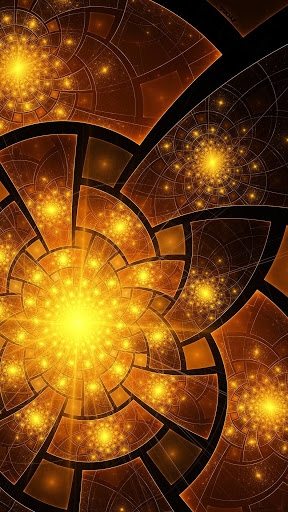
\includegraphics[width=\textwidth]{photos/cover1.jpg}}

\newcommand\BackgroundPic{%
\put(0,0){%
\parbox[b][\paperheight]{\paperwidth}{%
\vfill
\centering
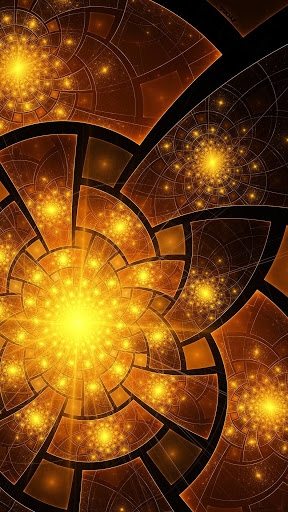
\includegraphics[width=\paperwidth,height=\paperheight,%
]{photos/cover1.jpg}%
\vfill
}}}

\begin{document}

\AddToShipoutPicture*{\BackgroundPic}
\color{white}
\maketitle
\color{black}
\newpage

\textit{Z dedykacją dla mojej ukochanej Zali.}
\newpage

\tableofcontents
\newpage


\section{Granica ciągu}

\subsection{Definicja}

\subsubsection{Definicja matematyczna}

\noindent
\textbf{Wersja ogólna}
\newline
Dla dowolnej przestrzeni o~dowolnej metryce (mierze odległości).
\newline
\newline
$ \exists_{g \in X} \lim_{n \to \infty} A(n) = g \iff \forall_{\epsilon>0} \exists_{N \in X} \forall_{n \geq N}  \rho(A(n), g) < \epsilon $
\newline
\newline
słownie: Ciąg A(n) dąży do~g z~przestrzeni~X przy~g dążącym do~nieskończoności wtedy i~tylko wtedy, gdy dla~dowolnego dodatniego~$\epsilon$ (czyt.~„epsilon”) istnieje~N należące do~przestrzeni~X takie, że~dla dowolnego~n większego od~N odległość ($\rho$, czyt.~„ro”) pomiędzy n-tym wyrazem ciągu~A a~liczbą~g jest mniejsza niż~$\epsilon$.
\newline

\noindent
\textbf{Wersja nam przydatna}
\newline
Czyli w~metryce euklidesowej dla~przestrzeni jednowymiarowej, tzn.~na~prostej z~liczbami rzeczywistymi, gdzie odległość między punktami liczymy wartością bezwzględną. 
\newline
\newline
$ \exists_{g \in \R} \lim_{n \to \infty} A(n) = g \iff \forall_{\epsilon>0} \exists_{N \in \R} \forall_{n \geq N} \left|A(n) - g\right| < \epsilon $
\newline
\newline
słownie: Ciąg A(n) dąży do~liczby~g z~przestrzeni~X przy g~dążącym do~nieskończoności wtedy i~tylko wtedy, gdy dla~dowolnego dodatniego~$\epsilon$ (czyt.~„epsilon”) istnieje liczba N taka, że~dla dowolnej liczby~n większej od~N różnica bezwzględna pomiędzy n-tym wyrazem ciągu~A a~liczbą~g jest mniejsza niż~$\epsilon$.
\newline

\noindent
\textbf{Inne nazewnictwa}
\begin{itemize}
    \item $\lim_{n \to \infty} A(n) = g$ możemy też zapisać w postaci \newline $A(n) \to g$ $(n \to \infty)$.
    \item Zamiast czytać „ciąg~A(n) dąży do~g przy~n dążącym do~nieskończoności” można również czytać „ciag~A(n) jest zbieżny do~g przy~n dążącym do~nieskończoności” lub „granica ciagu~A(n) przy~n dążącym do~nieskończoności wynosi~g”.
\end{itemize}
\indent

\subsubsection{Na chłopski rozum}
Mamy ciąg z~elementami ponumerowanymi indeksami 0, 1, 2, 3... (czyli A(0), A(1), A(2), A(3), ...). Ciąg taki dąży wartościami do~pewnej liczby~g, jeżeli –~ustaliwszy pewną dowolną małą liczbę (epsilon, $\epsilon$) –~znajdziemy taką liczbę~N, że~zarówno odległość między~A(N) a liczbą~g jest mniejsza od~naszej małej liczby~$\epsilon$, 
jak~i każdy następny wyraz jest odległy od~g o~mniej niż $\epsilon$. Wówczas prawie wszystkie wyrazy ciągu (wszystkie poza skończoną liczbą, tj.~od~0 do~N-1) znajdują się w~przedziale wartości $(g-\epsilon, g+\epsilon)$. 
Z~dowolności ustalenia epsilona wynika, że~w~nieskończoności te liczby dążą do~g, jak widać na~poniższym przykładzie.
\begin{figure}[H]
    \caption{Wykres ciagu A(n) = $(-1)^n * \frac{1}{n}$}
    \centering
        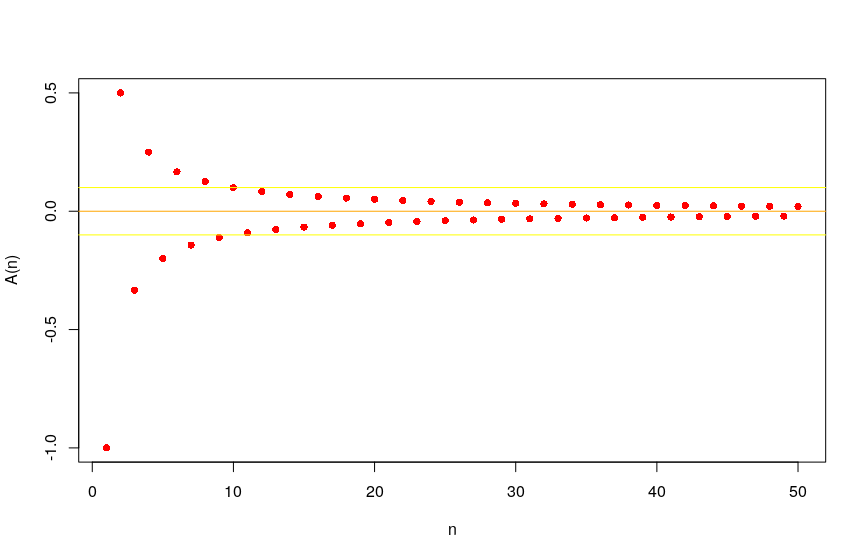
\includegraphics[width=0.75\textwidth]{photos/granica1.png}
\end{figure}
Widzimy, po~ustaleniu pewnej liczby $\epsilon$, że~prawie wszystkie wartości ciągu znajdują~się w~obrębie przedziału $(g-\epsilon, g+\epsilon)$ (zaznaczone jest to żółtymi prostymi), a~w~nieskończoności zbliżają~się do~liczby~g (zaznaczona pomarańczową prostą). Zatem ciąg~A(n) zbiega do~liczby~g.
W powyższym przypadku możemy zapisać to tak:
\begin{itemize}
    \item $A(n) = (-1)^n * \frac{1}{n} \to 0$ $(n \to \infty)$,
    \item $\lim_{n \to \infty} A(n) = (-1)^n * \frac{1}{n} = 0$.
\end{itemize} 

\subsection{Własności}

\subsection{Przykłady}

\subsection{Zadania}
\newpage

\section{Pochodne}
siema
\newpage

\section{Całki}
siema
\newpage
\AddToShipoutPicture*{\BackgroundPic}
koniec
\newpage

\end{document}